\documentclass[a4paper]{article}

%use the english line for english reports
%usepackage[english]{babel}
\usepackage[portuguese]{babel}
\usepackage[utf8x]{inputenc}
\usepackage{indentfirst}
\usepackage{graphicx}
\usepackage{verbatim}
\usepackage[top=2.5cm, bottom=3cm, left=2.5cm, right=2.5cm]{geometry}

\begin{document}

%\setlength{\textwidth}{16cm}
%\setlength{\textheight}{22cm}

\title{\Huge\textbf{Dominup em Prolog}\linebreak\linebreak\linebreak
\Large\textbf{Relatório Final}\linebreak\linebreak
\linebreak\linebreak

\includegraphics[scale=0.1]{feup-logo.png}\linebreak\linebreak
\linebreak\linebreak
\Large{Mestrado Integrado em Engenharia Informática e Computação} \linebreak\linebreak
\Large{Programação em Lógica}\linebreak
}

\author{\textbf{Dominup4:}\\
Ângela Filipa Pereira Cardoso - up200204375 \\
Nuno Miguel Rainho Valente - up200204376 \\
\linebreak\linebreak \\
 \\ Faculdade de Engenharia da Universidade do Porto \\ Rua Roberto Frias, s\/n, 4200-465 Porto, Portugal \linebreak\linebreak\linebreak
\linebreak\linebreak\vspace{1cm}}

\maketitle
\thispagestyle{empty}

%************************************************************************************************


\newpage

\section*{Resumo}

O trabalho por nós desenvolvido teve como principal objetivo a recriação de um jogo, o Dominup. Este é um jogo de tabuleiro sendo uma variação do famoso jogo de Dominó, aparentemente surgido na China há mais de dois mil anos.

O problema consisitiu em desenvolver o jogo em PROLOG SICSTUS e apresentar a sua interação com o utilizador na forma mais prática possível.

O Dominup será, posteriormente, alvo de maior detalhe neste relatório no que diz respeito a toda a sua jogabilidade, contudo, globalmente, permitimos que o jogo fosse jogado de três formas distintas:

\begin{itemize}
	\item Humano contra Humano.
	\item Humano contra Computador.
	\item Computador contra Computador.
\end{itemize}

Nos tipos de jogo que envolvem o computador foi necessário recorrer à implementação de inteligências artificiais, duas neste caso - uma mais simples e uma outra mais complexa.

%Resumo sucinto do trabalho com 150 a 250 palavras (problema abordado, objetivo, como foi o problema resolvido/abordado, principais resultados e conclusões).

\newpage

\tableofcontents

%************************************************************************************************
%************************************************************************************************
%************************************************************************************************
%************************************************************************************************

\newpage

%%%%%%%%%%%%%%%%%%%%%%%%%%
\section{Introdução}




O relatório está organizado por capítulos, sendo o primeiro correspondente a esta introdução.
No segundo capítulo fazemos uma apresentação detalhada do jogo Dominup com imagens ilustrativas que facilitam o entendimento do jogo.
Pretendemos dar a conhecer a lógica de jogo e a sua forma de implementação no jogo em Prolog.
% incluindo a forma de representação do estado do tabuleiro e sua visualização, execução de movimentos, verificação do cumprimento das regras do jogo, %determinação do final do jogo e cálculo das jogadas a realizar pelo computador utilizando diversos níveis de jogo. 
Toda esta informação está presente no capítulo três. Indicamos como funciona o módulo de interface com o utilizador em modo de texto - capítulo quatro, e fazemos alguns reparos finais nas conclusões - capítulo cinco. Terminamos com a bibliografia que utilizamos e em anexo apresentamos todo o código fonte do projeto.

%Descrever os objetivos e motivação do trabalho. Descrever num parágrafo breve a estrutura do relatório.


%%%%%%%%%%%%%%%%%%%%%%%%%%
\section{O Jogo Dominup}

Dominup é uma variação do jogo Dominó para 2 a 4 jogadores, em que, tal como o nome sugere, é possível colocar peças em cima de outras.

No típico Dominó existem 28 peças duplas numeradas de 0 a 6, à semelhança das faces de um dado. Já no Dominup há 36 peças duplas numeradas de 0 a 7, usando códigos binários: o ponto no centro representa 1, o circulo pequeno representa 2 e o circulo grande representa 4, como se pode ver na figura~\ref{piece}. Este desenho das peças, juntamente com as regras do Dominup e de dois outros jogos, foram criadas por Néstor Romeral Andrés em 2014, sendo o conjunto publicado por nestorgames\footnote[1]{http://www.nestorgames.com}.

\begin{figure}[htbp]
\begin{center}

\includegraphics[scale=0.5]{piece.jpg}
\caption{Exemplo da peça $3 \cdot 6$.}
\label{piece}
\end{center}
\end{figure}

Existem dois tipos de colocação de peças no Dominup:
\begin{itemize}
	\item subir - a peça é colocada em cima de duas peças adjacentes que estejam ao mesmo nível, de forma a que os números da peça colocada sejam iguais aos que ficam por baixo (um em cada peça de suporte), tal como mostra a figura~\ref{climb}.
	\item expandir - a peça é colocada na superfície de jogo, de forma a que fique adjacente e ortogonal a pelo menos uma peça já colocada, como, por exemplo, as duas peças já colocadas na figura~\ref{climb}.
\end{itemize}

\begin{figure}[htbp]
\begin{center}
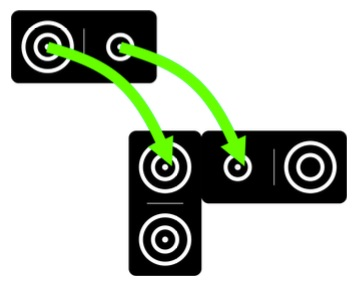
\includegraphics[scale=0.6]{climb.jpg}
\caption{Exemplo de um posicionamento a subir válido.}
\label{climb}
\end{center}
\end{figure}

Tal como no Dominó, as regras são relativamente simples. Começa-se por distribuir as peças aleatoriamente e de forma equilibrada pelos jogadores, mantendo a face voltada para baixo. 

O jogador com o duplo 7 inicia o jogo, colocando essa peça no centro da superfície de jogo e determinando a ordem dos restantes jogadores, que é dada pelo sentido contrário ao ponteiro dos relógios. 

Começando no segundo, cada jogador, na sua vez, realiza ambos os passos seguintes:
\begin{enumerate}
	\item Enquanto for possível, coloca peças a subir, podendo escolher a ordem em que o faz;
	\item Se ainda tiver alguma peça, coloca-a a expandir.
\end{enumerate}

Se, no final da sua vez, o jogador ficar sem peças, é declarado vencedor e o jogo termina. Alternativamente, os restantes jogadores podem continuar, de forma a determinar o segundo, terceiro e quarto lugares.

Na figura~\ref{example} pode ser observado um possível jogo de Dominup a decorrer.

\begin{figure}[htbp]
\begin{center}
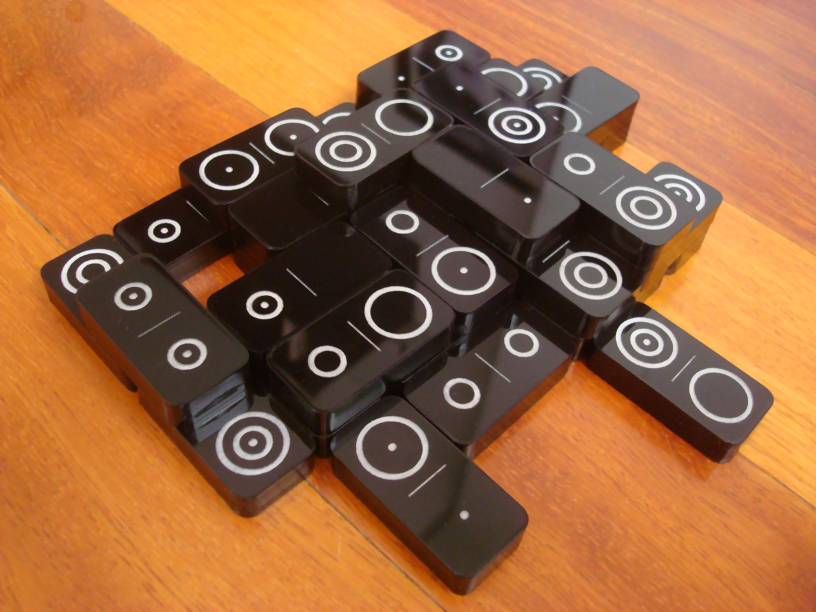
\includegraphics[scale=0.4]{example.jpg}
\caption{Exemplo de um jogo de Dominup.}
\label{example}
\end{center}
\end{figure}


%Descrever detalhadamente o jogo, a sua história e, principalmente, as suas regras.
%Devem ser incluidas imagens apropriadas para explicar o funcionamento do jogo.
%Devem ser incluidas as fontes de informação (e.g. URLs em rodapé).

%%%%%%%%%%%%%%%%%%%%%%%%%%
\section{Lógica do Jogo}

Descrever o projeto e implementação da lógica do jogo em Prolog, incluindo a forma de representação do estado do tabuleiro e sua visualização, execução de movimentos, verificação do cumprimento das regras do jogo, determinação do final do jogo e cálculo das jogadas a realizar pelo computador utilizando diversos níveis de jogo. Sugere-se a estruturação desta secção da seguinte forma:

\subsection{Representação do Estado do Jogo} Pode ser idêntico ao descrito no relatório intercalar.)

\subsection{Visualização do Tabuleiro} (Pode ser idêntico ao descrito no relatório intercalar.)

\subsection{Lista de Jogadas Válidas} Obtenção de uma lista de jogadas possíveis. Exemplo: \textit{valid\_moves(+Board, -ListOfMoves)}.

\subsection{Execução de Jogadas} Validação e execução de uma jogada num tabuleiro, obtendo o novo estado do jogo. Exemplo: \textit{move(+Move, +Board, -NewBoard)}.

\subsection{Avaliação do Tabuleiro} Avaliação do estado do jogo, que permitirá comparar a aplicação das diversas jogadas disponíveis. Exemplo: \textit{value(+Board, +Player, -Value)}.

\subsection{Final do Jogo} Verificação do fim do jogo, com identificação do vencedor. Exemplo: \textit{game\_over(+Board, -Winner)}.

\subsection{Jogada do Computador} Escolha da jogada a efetuar pelo computador, dependendo do nível de dificuldade. Por exemplo: \textit{choose\_move(+Level, +Board, -Move)}.

- uma mais simples que de entre as jogadas válidas seleciona uma qualquer, e uma outra mais complexa que avalia para cada jogada possível qual a mais eficaz para levar o computador a vencer.




%%%%%%%%%%%%%%%%%%%%%%%%%%
\section{Interface com o Utilizador}

Descrever o módulo de interface com o utilizador em modo de texto.


%%%%%%%%%%%%%%%%%%%%%%%%%%
\section{Conclusões}

Este jogo foi desde logo uma das nossas primeiras hipóteses de seleção, de entre quatro possíveis, para se desenvolver o primeiro projeto em Prolog que seria objeto de avaliação. Ficamos extremamente felizes com o desenvolvimento de um jogo que à partida trazia alguma nostalgia pelo simples facto de nos lembrar alguns momentos, em que outrora um simples jogo de Dominó fazia a delícia dos mais pequenos. 

Somos da opinião que este jogo trás uma espécie de reformulação do típico jogo de dominó e que faz todo o sentido coloca-lo disponível a jogar num computador, apesar de ainda em modo de texto.

Relativamente ao projeto consideramos que tudo o que delineamos e que todos os pontos exigidos na implementação do jogo foram cumpridos. Foi muito proveitoso uma vez que serviu também para praticarmos e aumentarmos a nossa prática em programação lógica.

Gostaríamos de ter desenvolvido mais um nível de inteligência artificial e ter colocado a dimensão do tabuleiro de jogo a ser adaptado dinamicamente, isto é, consoante a colocação de peças e os movimentos de expand,o tabuleiro ir aumentando de dimensão.

Todavia, estamos agradados com o rumo que o porjeto tomou e o resultado final foi o que esperavamos.

%Que conclui deste projecto? Como poderia melhorar o trabalho desenvolvido?


\clearpage
\addcontentsline{toc}{section}{Bibliografia}
\renewcommand\refname{Bibliografia}
\bibliographystyle{plain}
\bibliography{myrefs}
\begin{itemize}
	\item http://www.nestorgames.com
	\item https://sicstus.sics.se/sicstus/docs/4.0.3/html/sicstus/Saving.html
	\item https://sicstus.sics.se/sicstus/docs/latest4/pdf/sicstus.pdf
	\item Apontamentos das aulas teóricas
\end{itemize}

\newpage
\appendix
\section{Código fonte do jogo Dominup}
Apresenta-se a seguir todo o código fonte utilizado no projeto:
%Código Prolog implementado devidamente comentado e outros elementos úteis que não sejam essenciais ao relatório.

\end{document}
